%!TEX options = --shell-escape
%!TEX program = lualatex
\documentclass[12pt,a4paper,twoside]{uiothesis}
\usepackage[english]{babel}
\author{John Doe}

% Titlepage
\makeatletter
\renewcommand{\maketitle}{%
  \begin{titlingpage}
    \begin{centered}
        \null\vspace{8pc}

        {\Huge\color{title}\uppercaps{Awesome Stuff}} \\
        \vspace{2pc}
        {\Huge\textit{{about}}} \\
        \vspace{2pc}
        {\Huge\color{title}\uppercaps{Things}} \\

        \vspace{4pc}
        {\Large\aldineleft} \\
        \vspace{4pc}

        {\Large\textit{{
          Very interesting paper  \\
          \vspace{1pc}
          about awesome stuff}}} \\

        \vspace{5pc}

        {\large\@author} \\

        \vspace{2pc}

        {\large June 2021} \\

        \vspace{5pc}

        \textit{
        Thesis\\
        \vspace{1pc}
        at the \\
        \vspace{1pc}
        University of Glennkill \\
        faculty of electrical engineering\\
        }
        \vfill
        \@scm
    \end{centered}
    \cleardoublepage
    \makecolophon
  \end{titlingpage}
}
\makeatother


\setlength{\emergencystretch}{1em}
\usepackage{xcolor}
\usepackage{caption}

\usepackage{csquotes}
\usepackage{graphicx}
\usepackage{pgfplots}
\pgfplotsset{compat=1.13}

\usepackage{blindtext}

\begin{document}
\chapterstyle{uio}
\pagestyle{uio}
\maxsecnumdepth{subsection}

\frontmatter
\pagenumbering{alph}
\maketitle
% \part{Preface}
\pagenumbering{roman}
\clearpage
\include{abstract}
\cleardoublepage
\tableofcontents
\clearpage
\listoffigures
\clearpage
% \listoftables
% \listofsourcecode
\mainmatter

\chapter{Awesome Chapter}
\blindtext
\section{Here is a awesome chart}

The bar chart is from \url{http://tex.stackexchange.com/questions/46316/how-to-put-the-values-of-each-bar-in-a-pgfplots-bar-chart-inside-the-bar-itself}. It is awesome.
\begin{figure}[ht!]

\begin{margincap}
\begin{tikzpicture}
\begin{axis}[
compat=newest, %Better label placement
ybar = 0.6,
width=\textwidth,
height=0.3\textheight,
enlarge y limits={upper, value=0.2},
ymin=0,
enlarge x limits = 0.2,
bar width=32pt,
title={Instance els19 with 1\% max error},
legend style={at={(0.5,-0.15)},
anchor=north,legend columns=0},
ylabel={Time in milisseconds},
symbolic x coords={s-HAS, s-cAS, CUDA-HAS},
xtick=data,
nodes near coords,
axis lines*=left,
y axis line style={opacity=0},
yticklabels={\empty},
ytick style={draw=none},
cycle list={
    {fill=black!60,draw=black!60},
    {fill=black!40,draw=black!40},
    {fill=black!20,draw=black!20}
},
axis on top,
major grid style=white,
ymajorgrids,
legend style={draw=none,/tikz/every even column/.append style={column sep=0.5cm}}
]
\addplot coordinates {(s-HAS,4) (s-cAS,4) (CUDA-HAS,6)};
\addplot coordinates {(s-HAS,44.60) (s-cAS,71.90) (CUDA-HAS,8.67)};
\addplot coordinates {(s-HAS,156) (s-cAS,334) (CUDA-HAS,18)};
\legend{Best 1\%,Average 1\%,Worst 1\%}
\end{axis}
\end{tikzpicture}
\caption{It is \emph{really} awesome -- believe me. It shows something with gray bars, but I've no idea what exactly it is about.}

\end{margincap}
\end{figure}

\blindtext
\blinddocument

\end{document}
